\chapter{Divide et Impera}
\section{Enun't}
\myindent
Se d'a un pachet de 52 de c'ar'ti de joc. Pachetul nu con'tine Jokeri. Se citesc din fisierul "Pachet carti.in" cele 4 tipuri de c'ar'ti 'intr-o ordine aleatoare urmat'a de num'arul 'si tip-ul unei c'ar'ti din pachet. Toate c'ar'tile vor fi aranjate 'in ordine cresc'atoare 'si 'in ordinea tipurilor a'sa cum este dat'a din fisierul de intrare. As-ul va fi considerat num'arul 11. S'a se g'aseasc'a pozi'tia c'ar'tii citite de la input.
\newline
\newline
\myindent
Pentru aceast'a problem'a avem urm'atoarele nota'tii: ir - inim'a ro'sie; in - inim'a neagr'a; rb - romb; tr - trefl'a.
\vspace{15mm}

\section{Descrierea solu'tiei problemei}
\vspace{10mm}
\myindent
Problema dat'a se poate rezolva folosind un algortim de c'autare. Av\^and avantajul c'a toate c'ar'tile de un tip sunt sortate putem apela la o c'autare binar'a, 'ins'a tipurile nu sunt sortate si nici nu pot fi sortate 'in vreun fel pentru a putea aplica c'autarea binar'a peste tot pachetul, a'sa c'a se va recurge la un compromis.\\
\newline
\myindent
La 'inceputul programului se vor citi datele de intrare 'si se va forma un vector de structuri. Pentru aceast'a metod'a se va folosi structura carte ce con'tine un int pentru num'arul c'ar'tii 'si un string pentru tipul c'ar'tii. Dup'a formarea vectorului se va apela func'tia Find\_Card care va c'auta 'intr-o prim'a etap'a tipul c'ar'tii 'si apoi va c'auta dup'a num'ar. Func'tia prime'ste vectorul, dar 'si indicii de 'inceput 'si sf\^ar'sit ai vectorului, verific'a mijlocul vectorului 'si 'imparte problema 'in dou'a sau 'imparte pachetul 'in dou'a p'ar'ti cu caracteristici diferite. Odat'a cu g'asirea tipului, algoritmul ajunge la eficien'ta cea mai bun'a 'intruc\^at aceast'a bucat'a de vector este ordonat'a cresc'ator. Aplic\^andu-se algoritmul de c'autare binar'a ajungem rapid la cartea c'autat'a 'si 'in final se va afi'sa pozi'tia g'asit'a.

\vspace{10mm}
\section{Prezentarea algoritmului de rezolvare a problemei}

\begin{lstlisting}[language=Python]
structura{
	numar;
	tip;
} carte

int Find_card(pachet, carte, start, end)
	daca start > finish
		daca pachet[start] == carte
			returneaza start;
	
		altfel returneaza -1;

	mid = (start + finish) / 2;
	
	daca pachet[mid] == carte
		returneaza mid;

	daca tipul lui carte == tip pachet[start] si tip pachet[finish]
		daca numar carte < numar pachet[mid]
			returneaza Find_card(pachet, carte, start, mid-1);

		returneaza Find_card(pachet, carte, mid + 1, finish);

	left = Find_card(pachet, carte, start, mid - 1);
	right = Find_card(pachet, carte, mid + 1, finish);

	daca left diferit de -1
		returneaza left;

	returneaza right;


int main()
	citeste n
	pentru i de la 1 la n
		citeste type 
		
		pentru j de la 0 la 13
			pachet[j + i * 13] = carte(j + 2, type);

	citeste searched;
	scrie Find_Card(pachet, searched, 0 , 51) + 1;
	returneaza 0;
\end{lstlisting}

\vspace{10mm}
\section{Aprecierea complexit'a'tii algoritmului propus}
\myindent
Complexitatea algoritmului dat pentru un singur pachet de 52 de c'ar'ti este O(1) deoarece avem un num'ar fix de c'ar'ti, deci un num'ar fix de tipuri de c'ar'ti, astfel vom avea un num'ar finit de intruc'tiuni executate. Pentru mai multe pachete de c'ar'ti puse toate 'intr-un singur loc algoritmul va avea complexitatea O(n) deoarece c\^and se intr'a 'in Find\_cards 'int\^ai se va aplica c'autarea binar'a pe tot pachetul p\^an'a c\^and se va ajunge la un set cu tipul respectiv, ceea ce va scoate o complexitate O(n), iar c'autarea pe un singur set va scoate O(1) deoarece setul are un num'ar fix de c'ar'ti. Dac'a set-urile nu ar avea valori fixe algortimul ar scoate o complexitate O(log m) unde m este num'arul de c'ar'ti dintr-un set deoarece s-ar fac face c'autare binar'a pe un 'sir cresc'ator. Deci, complexitatea 'in cel mai r'au caz este O(n).

\vspace{5mm}
\section{Analiza succint'a asupra eficien'tei algoritmului propus}
\myindent
Acest algoritm, desi este eficient din punct de vedere al timpului de execu'tie, complexitatea spa'tial'a ar fi O(n) deoarece s-ar genera c\^ate dou'a apeluri de func'tii pentru fiecare tip de carte p\^an'a la g'asirea tipului c'ar'tii. Modalitatea prin care s-ar putea sc'apa de aceast'a complexitate este folosirea unei formule matematice, dar asta ar 'insemna s'a nu folosim metoda Divide et Impera. Deci, algoritmul folosit pentru rezolvarea acestei probleme este optim 'in m'asura 'in care se cere 'in cerin't'a rezolvarea doar cu Divide et Impera.

\vspace{10mm}
\section{Exemplificarea aplic'arii algoritmului propus pentru un exemplu sugestiv}
\subsection{Exemplu de input}
\begin{verbatim}
Pachet carti.in
4
ir
in
rb
tr
8 tr

Rezultatul: 46
\end{verbatim}

\subsection{Aplicarea algoritmului}
\begin{figure}[H]
\centering
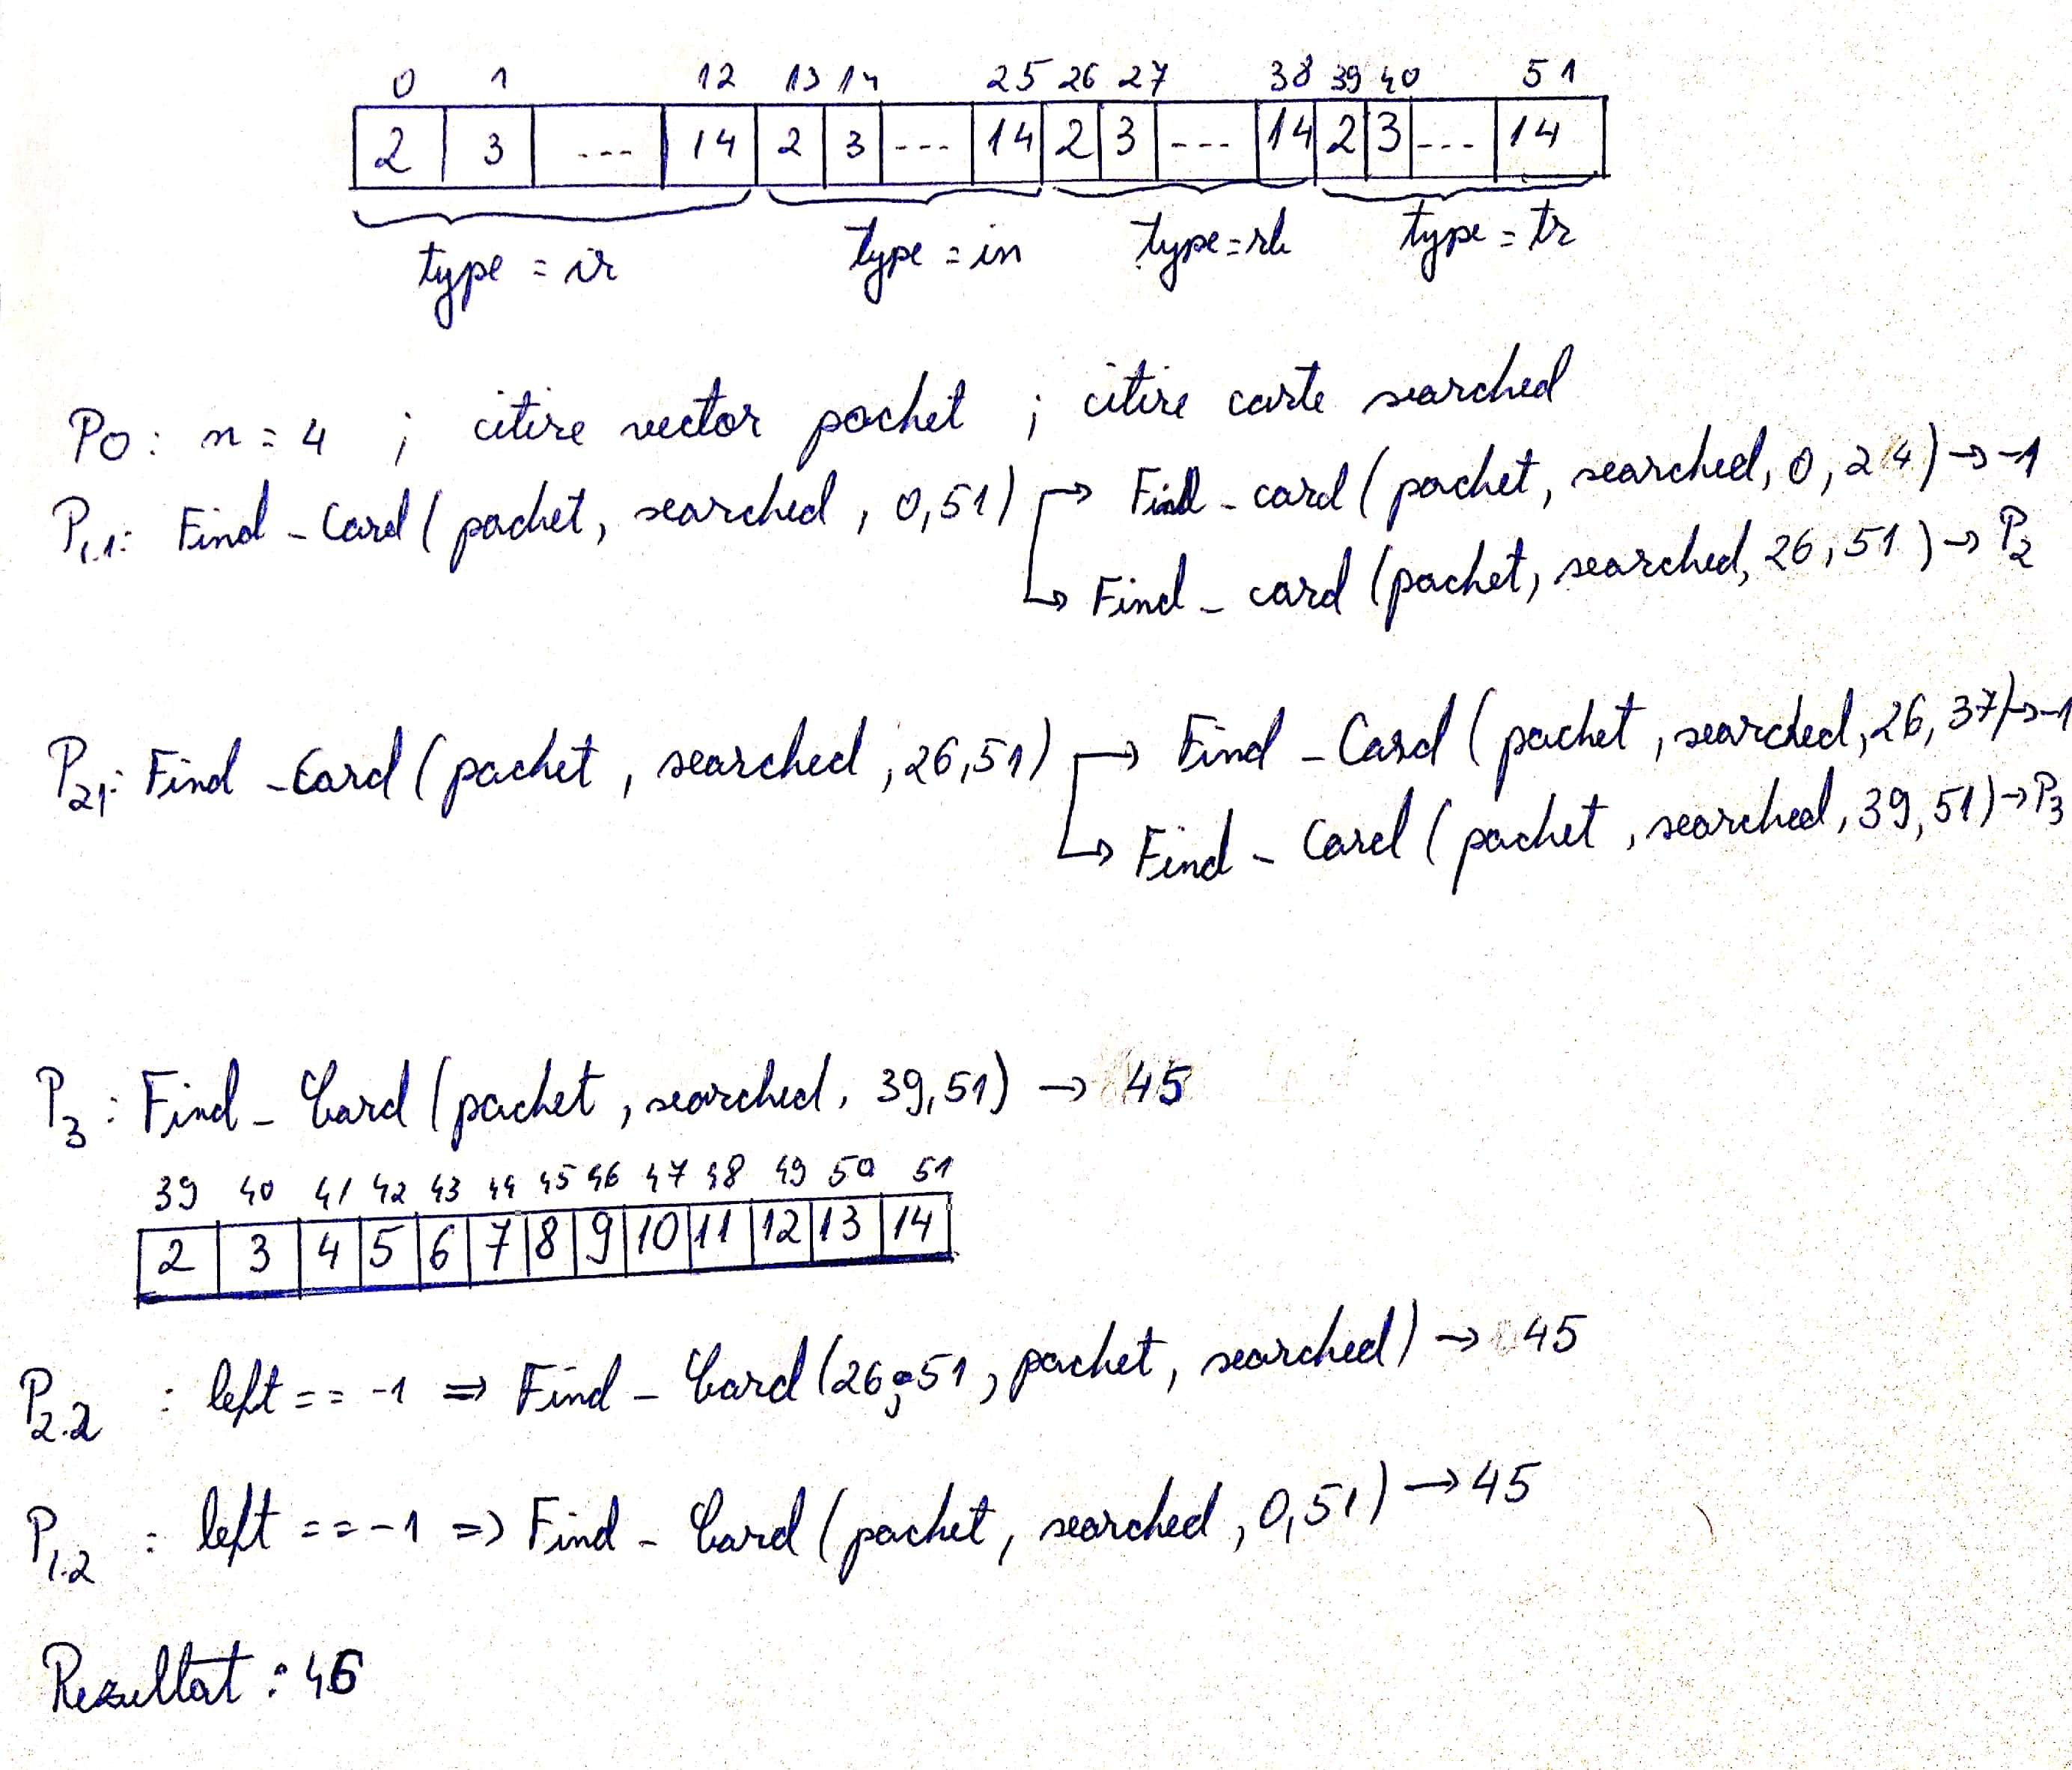
\includegraphics[scale = 0.17]{Divide et Impera/Exemplu}
\end{figure}
\vspace{10mm}
Pasul 0: Se cite'ste din fi'sierul de intrare n 'si cele n tipuri de c'ar'ti, se creeaz'a vectorul pachet 'si se citesc datele c'ar'tii c'autate (8 de trefl'a). Se apeleaz'a func'tia Find\_Card pe tot pachetul.\\
\newline
Pasul 1.1: Se verific'a dac'a mijlocul pachetului este cartea c'autat'a 'si 'in acest caz nu este. Tipul c'ar'tii de la indicele start nu este trefl'a, deci se va apela de dou'a ori Find\_Card, odat'a pe c'ar'tile de la pozi'tiile 0-24, apel care va returna -1 pentru c'a acea bucat'a nu con'tine 8-ul de trefl'a si 'inc'a odata pe c'ar'tile de la 26 la 37.\\
\newline
Pasul 2.1: Se verific'a mijlocul pachetului 'si observam ca din nou nu se potrive'ste, se mai observ'a c'a tipul c'ar'tii de la indicele start nu este trefl'a, deci se apeleaz'a din nou Find\_Card de 2 ori. Primul apel va returna -1 deoarece toate c'ar'tile acoperite de func'tie, adic'a 26-37 sunt de romb. Al doilea apel va acoperi toate c'artile de trefl'a, adic'a 39-51.\\
\newline
Pasul 3: Se verific'a mijlocul 'si se constat'a o potrivire 'intre cartea c'autat'a 'si cartea de la pozi'tia 45. Se va returna 45.\\
\newline
Pasul 2.2: Apelul din variabila left nu con'tine solu'tia, deci va returnat -1 care condi'tioneaz'a programul s'a returneze 45.\\
\newline
Pasul 1.2: Partea st\^ang'a a pachetului nu con'tine cartea c'autat'a ceea ce 'inseamn'a c'a partea dreapt'a o con'tine. Se returneaz'a 45.\\
\newline
Se va scrie 'in output rezultatul func'tiei Find\_Card + 1, adic'a 46 pentru c'a num'ar'atoarea in program a 'inceput de la 0 'si 'in realitate ea 'incepe de la 1.